\documentclass{beamer}
\usetheme{Madrid}
\usepackage{graphicx}
\usepackage{hyperref}
\usepackage{listings}
\usepackage{xcolor}

\title{PairCoder: Agent Collaboration for Smarter Code Generation}
\author{Taylan Bapur}
\institute{Machine Learning in Software Engineering Seminar}
\date{2025}

\definecolor{codegray}{rgb}{0.5,0.5,0.5}
\lstdefinestyle{mystyle}{
    backgroundcolor=\color{white},
    commentstyle=\color{gray},
    keywordstyle=\color{blue},
    numberstyle=\tiny\color{codegray},
    stringstyle=\color{red},
    basicstyle=\ttfamily\footnotesize,
    breakatwhitespace=false,
    breaklines=true,
    captionpos=b,
    keepspaces=true,
    numbers=left,
    numbersep=5pt,
    showspaces=false,
    showstringspaces=false,
    showtabs=false,
    tabsize=2
}
\lstset{style=mystyle}

\begin{document}

\frame{\titlepage}

% Introduction
\begin{frame}{Motivation}
\begin{itemize}
  \item LLMs can generate code but struggle with complex logic
  \item Rigid, single-path plans limit robustness
  \item Human pair programming inspires agent collaboration
\end{itemize}
\end{frame}

% Framework
\begin{frame}{What is PairCoder?}
\begin{itemize}
  \item Two LLM agents: \textbf{Navigator} and \textbf{Driver}
  \item Navigator reflects, plans, selects strategies
  \item Driver implements, tests, and refines code
  \item Agents work in an iterative feedback loop
\end{itemize}
\end{frame}

% System Architecture Figure
\begin{frame}{PairCoder Architecture}
\centering
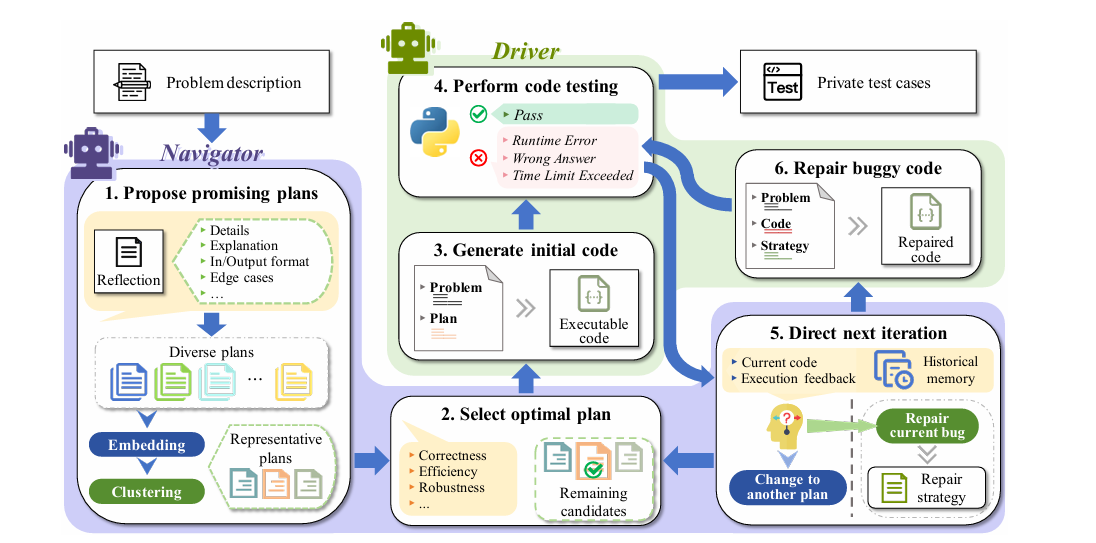
\includegraphics[width=0.85\textwidth]{paircoder-architecture.png} \\[0.5em]
\small Source: Zhang et al. (2024)
\end{frame}

% Key Techniques
\begin{frame}{Key Techniques}
\begin{itemize}
  \item \textbf{Multi-Plan Exploration}: Generate, cluster, and select diverse plans
  \item \textbf{Feedback-Driven Refinement}: Use test results to refine or switch strategies
  \item Historical memory to avoid redundant attempts
\end{itemize}
\end{frame}

% Driver Code Snippet
\begin{frame}[fragile]{Example: Initial Code by Driver}
\begin{lstlisting}[language=Python,caption=Driver's original code output]
def solve(arr):
    operations = 0
    for i, val in enumerate(arr):
        if val > i + 1:
            operations += val - (i + 1)
    return operations
\end{lstlisting}
\end{frame}

% Feedback Fix Code
\begin{frame}[fragile]{Refined Code after Feedback}
\begin{lstlisting}[language=Python,caption=Code after Navigator refinement]
def solve_fixed(arr):
    arr = arr[:]
    i = 0
    ops = 0
    while i < len(arr):
        if arr[i] > i + 1:
            arr.insert(i, i + 1)
            ops += 1
        else:
            i += 1
    return ops
\end{lstlisting}
\end{frame}

% Benchmarks
\begin{frame}{Results and Benchmarks}
\begin{itemize}
  \item Datasets: HumanEval, MBPP, CodeContest
  \item Up to 162\% improvement in pass@1 over baselines
  \item PairCoder excels at complex tasks requiring logical precision
\end{itemize}
\end{frame}

% Accuracy Figure
\begin{frame}{Accuracy Gains (pass@1)}
\centering
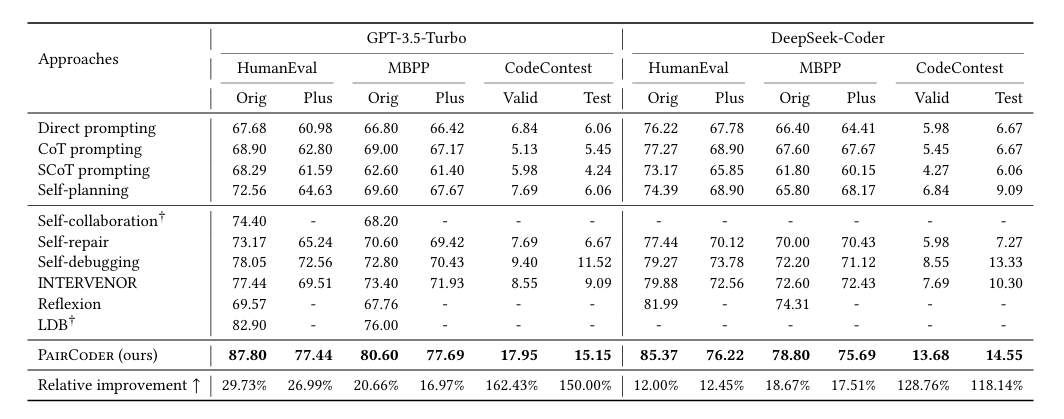
\includegraphics[width=0.8\textwidth]{paircoder-results.png} \\[0.5em]
\small Source: Zhang et al. (2024)
\end{frame}

% Ablation
\begin{frame}{Ablation and Efficiency}
\begin{itemize}
  \item Removing Multi-Plan drops accuracy by 6--8\%
  \item Removing Feedback Loop drops it by 10--12\%
  \item Balance of performance vs. token/API cost
\end{itemize}
\end{frame}

% Comparison
\begin{frame}{PairCoder vs. MapCoder}
\begin{itemize}
  \item \textbf{PairCoder}: 2 tightly-coupled agents for focused refinement
  \item \textbf{MapCoder}: full pipeline (retrieval, planning, generation, debugging)
  \item PairCoder = Agile; MapCoder = Comprehensive
\end{itemize}
\end{frame}

% Limitations
\begin{frame}{Limitations and Future Work}
\begin{itemize}
  \item Performance depends on initial plan quality
  \item Computationally expensive in real-time contexts
  \item Extend with human-in-the-loop or automated test generation
\end{itemize}
\end{frame}

% Conclusion
\begin{frame}{Conclusion}
\begin{itemize}
  \item PairCoder leverages agent collaboration for robust code generation
  \item Outperforms state-of-the-art baselines
  \item Paves the way for agentic software engineering tools
\end{itemize}
\end{frame}

% Q&A
\begin{frame}{Questions?}
\centering
\Large Thank you!\newline
Questions and discussion welcome.
\end{frame}

\end{document}